%https://tex.stackexchange.com/questions/164991/pgfplots-how-to-fill-bounded-area-under-a-curve-using-addplot-and-fill

%https://tex.stackexchange.com/questions/140312/tikz-shading-region-bounded-by-several-curves
%tikz para graficar areas

%http://latexcolor.com/

%https://www.tablesgenerator.com/
\PassOptionsToPackage{force}{filehook}

\documentclass{beamer}


\usepackage[utf8]{inputenc}
\usepackage{amsmath}
\usepackage{amssymb}% http://ctan.org/pkg/amssymb
\usepackage{amsfonts}
\usepackage{pifont}% http://ctan.org/pkg/pifont
%https://tex.stackexchange.com/questions/42619/x-mark-to-match-checkmark
\newcommand{\cmark}{\ding{51}}
\newcommand{\xmark}{\ding{55}}
%\usepackage{amsfonts}
\usepackage{graphicx} 
\usepackage{subcaption}
\usepackage{hyperref}
\usepackage{cancel}
\usepackage{wrapfig}
\usepackage{enumitem}
\usepackage{comment}
\hypersetup{
	colorlinks=true,
	linkcolor=blue,
	filecolor=magenta,      
	urlcolor=cyan,
}
\newtheorem*{proposicion}{Proposici\'on}
\newtheorem*{teorema}{Teorema}
\renewcommand*{\proofname}{Demostraci\'on}
\newtheorem*{ejercicio}{Ejercicio}
\usepackage{pgf,tikz}
\usetikzlibrary{positioning}
\usetikzlibrary{arrows,patterns}
\usetikzlibrary{arrows.meta}
\usepackage[spanish, activeacute]{babel} %Definir idioma español
\usepackage[utf8]{inputenc} %Codificacion utf-8
\usepackage{multirow}

%   Esconder las soluciones
\newif\ifhideproofs
\hideproofstrue %uncomment to hide proofs

\ifhideproofs
\usepackage{environ}
\NewEnviron{hide}{}
\let\solucion\hide
\let\endsolucion\endhide
\fi

\usepackage{color}
\usepackage{mathpazo}
\usepackage{hyperref}
\usepackage{multimedia}
\usepackage{graphicx}
\usepackage{textcomp}
\usepackage[spanish, activeacute]{babel} 
\usepackage{graphicx} 
\usepackage{booktabs}
\usepackage{cite}
\usepackage{hyperref}
\usepackage{multicol}
\usepackage{multirow,array}

\usepackage{mathrsfs}
%\usepackage{amssymb}

\usepackage{tabularx}
    \newcolumntype{L}{>{\raggedright\arraybackslash}X}
        %\newcolumntype{b}{>{\hsize=1.5\hsize}X}
    %\newcolumntype{s}{>{\hsize=.9\hsize}X}

\usepackage{amsthm}
\newtheorem{thm}{Teorema}
\newtheorem{lem}[thm]{Lema}
\newtheorem{axiom}[thm]{Axioma}
\newtheorem{prop}[thm]{Proposici\'on}
\newtheorem{coro}[thm]{Corolario}
\theoremstyle{definition}
\newtheorem{defn}{Definici\'on}
\DeclareGraphicsExtensions{.pdf,.jpeg,.png,.eps}
\usetheme{CambridgeUS}
\setbeamertemplate{navigation symbols}{}

%Paréntisis y otros
\newcommand{\cmc}{\overset{m.c.}{\rightarrow}}
\newcommand{\p}[1]{\left(#1\right)}
\newcommand{\cor}[1]{\left[#1\right]}
\newcommand{\lla}[1]{\left\{#1\right\}}
\newcommand{\eps}{\varepsilon}
\newcommand{\lol}{\mathcal{L}}
\newcommand{\RR}{\mathbb{R}}
\newcommand{\QQ}{\mathbb{Q}}
\newcommand{\NN}{\mathbb{N}}
\newcommand{\paren}[1]{\left(#1\right)}
\newcommand{\corc}[1]{\left[#1\right]}
\newcommand{\llav}[1]{\left\lbrace#1\right\rbrace}
\newcommand{\partt}[1]{\left(\text{#1}\right)}
\newcommand{\corctt}[1]{\left[\text{#1}\right]}
\newcommand{\llavtt}[1]{\left\lbrace\text{#1}\right\rbrace}
\makeatletter
\def\munderbar#1{\underline{\sbox\tw@{$#1$}\dp\tw@\z@\box\tw@}}
\makeatother

%\usepackage[scr=rsfs,cal=boondox]{mathalfa}
\usepackage[scr=esstix,cal=boondox]{mathalfa}

% \usepackage{mdframed}
% \newmdtheoremenv{solucion}{Soluci\'on}

% Enmarcar las soluciones
% \newenvironment{solu}
% {%
% \begin{framed}
%   \begin{solucion}
%   }%
%     {%     
%   \end{solucion}
% \end{framed}
% }

%   Esconder las soluciones
\newif\ifhideproofs
%\hideproofstrue %uncomment to hide proofs

\ifhideproofs
\usepackage{environ}
\NewEnviron{hide}{}
\let\solucion\hide
\let\endsolucion\endhide
\fi



%Graficos y cosas
\usepackage{amssymb}
\usepackage{tikz}
\usepackage{pgfplots}
\usepackage{mathtools}
\usepackage{xcolor}
%\pgfplotsset{compat=1.9}
\usepgfplotslibrary{fillbetween,decorations.softclip}
\pgfplotsset{compat = newest}
\usepackage{pst-func}
\usepackage{pstricks}
\usepackage{pst-plot}

% Comando para usar multiples footnotes en un align environment

\makeatletter
\newcommand{\AlignFootnote}[1]{%
    \ifmeasuring@
    \else
        \footnote{#1}%
    \fi
}
\makeatother

%https://tex.stackexchange.com/questions/82782/footnote-in-align-environment


\DeclareGraphicsExtensions{.pdf,.jpeg,.png,.eps}
\usepackage{tikz}
%\usepackage{tikz-cd}
\usetikzlibrary{decorations}
%\usetikzlibrary{snakes}
\usetikzlibrary{cd}

\useoutertheme{split}
\useinnertheme{rounded}


%\beamertemplatenavigationsymbolsempty  %removes navigation bar
\definecolor{rosee}{rgb}{0.7,0.05,0.25}
\definecolor{pacificorange}{cmyk}{0,.6,1,0} %approved Pacific colors 2010
\definecolor{pacificgray}{cmyk}{0,.15,.35,.60}
\definecolor{pacificlgray}{cmyk}{0,0,.2,.4}
\definecolor{pacificcream}{cmyk}{.05,.05,.15,0}
\definecolor{deepyellow}{cmyk}{0,.17,.80,0}
\definecolor{lightblue}{cmyk}{.49,.01,0,0}
\definecolor{lightbrown}{cmyk}{.09,.15,.34,0}
\definecolor{deepviolet}{cmyk}{.79,1,0,.15}
\definecolor{deeporange}{cmyk}{0,.59,1,18}
\definecolor{dustyred}{cmyk}{0,.7,.45,.4}
\definecolor{grassgreen}{RGB}{92,135,39}
\definecolor{pacificblue}{RGB}{59,110,143}
\definecolor{pacificgreen}{cmyk}{.15,0,.45,.30}
\definecolor{deepblue}{cmyk}{1,.57,0,2}
\definecolor{turquoise}{cmyk}{.43,0,.24,0}
\definecolor{gren}{rgb}{0.2,0.8,0.5}
\definecolor{orang}{rgb}{1,0.64,0}
\definecolor{amethyst}{rgb}{0.6, 0.4, 0.8}
\definecolor{dodgerblue}{rgb}{0.12, 0.56, 1.0}
\definecolor{fandango}{rgb}{0.71, 0.2, 0.54}
\definecolor{forestgreen(traditional)}{rgb}{0.0, 0.27, 0.13}
\definecolor{iris}{rgb}{0.35, 0.31, 0.81}
\definecolor{jazzberryjam}{rgb}{0.65, 0.04, 0.37}
\definecolor{mediumjunglegreen}{rgb}{0.11, 0.21, 0.18}
\definecolor{mediumpersianblue}{rgb}{0.0, 0.4, 0.65}
\definecolor{midnightgreen}{rgb}{0.0, 0.29, 0.33}
\definecolor{orangee}{rgb}{1.0, 0.5, 0.0}

% There are many different themes available for Beamer. A comprehensive
% list with examples is given here:
% http://deic.uab.es/~iblanes/beamer_gallery/index_by_theme.html
% You can uncomment the themes below if you would like to use a different
% one:
%\usetheme{AnnArbor} %boca
%\usetheme{Antibes} %azul y gris
%\usetheme{Bergen} %barra who where
%\usetheme{Berkeley} %bordes
%usetheme{Berlin} %blanco y azul
%\usetheme{Boadilla}
%\usetheme{boxes}
\usetheme{CambridgeUS}
%\usetheme{Copenhagen}
%\usetheme{Darmstadt}
%\usetheme{default}
%\usetheme{Frankfurt}
%\usetheme{Goettingen}
%\usetheme{Hannover}
%\usetheme{Luebeck}
%\usetheme{Malmoe}
%\usetheme{Marburg}
%\usetheme{Montpellier}
%\usetheme{PaloAlto}
%\usetheme{Pittsburgh}
%\usetheme{Rochester}
%\usetheme{Singapore}
%\usetheme{Szeged}
%\usetheme{Warsaw}

%\usecolortheme{beaver}
%\usecolortheme{whale}
%\usecolortheme{orchid}
%\usecolortheme{wolverine}
%\usecolortheme[named=pacificblue]{structure} %replaces the blue of Copenhagen with Pacific orange

\definecolor{myNewColorA}{rgb}{0,0,100}
\definecolor{myNewColorB}{rgb}{0,100,100}
\definecolor{myNewColorC}{rgb}{0,200,100}
\definecolor{myNewColorD}{rgb}{0,100,200}

%\setbeamercolor*{palette primary}{bg=myNewColorA, fg = black}
%\setbeamercolor*{palette secondary}{bg=myNewColorB, fg = black}
%\setbeamercolor*{palette tertiary}{bg=myNewColorC, fg = black}
%\setbeamercolor*{palette quaternary}{bg=myNewColorD, fg = black}

\setbeamercolor*{palette primary}{bg=rosee, fg = white}
\setbeamercolor*{palette secondary}{bg=gren, fg = white}
\setbeamercolor*{palette tertiary}{bg=-red!75!, fg = white}
\setbeamercolor*{palette quaternary}{bg=-red!75!, fg = white}

\newtheorem{proposition}{Proposici\'on}
\newcommand{\ton}{\underset{n\to\infty}{\longrightarrow}}
\newcommand{\cp}{\overset{P}{\rightarrow}}
\newcommand{\cw}{\overset{d}{\rightarrow}}

%\expandafter\def\expandafter\insertshorttitle\expandafter{%
 % \insertshorttitle\hfill%
  %\insertframenumber\,/\,\inserttotalframenumber}

%\mode
%<all>

%Para agrandar el espacio entre renglones de las tablas
%https://tex.stackexchange.com/questions/26690/how-to-add-extra-spaces-between-rows-in-tabular-environment
\renewcommand{\arraystretch}{1.5}

\usepackage{color, xcolor}
\definecolor{codegreen}{rgb}{0,0.6,0}
\definecolor{codegray}{rgb}{0.5,0.5,0.5}
\definecolor{codepurple}{rgb}{0.58,0,0.82}
\definecolor{backcolour}{rgb}{0.95,0.95,0.92}

\usepackage{listings}
\lstdefinestyle{mystyle}{
  backgroundcolor=\color{backcolour},   
  commentstyle=\color{codegreen},
  language = R,
  % commentchar=\#,
  keywordstyle=\color{magenta},
  numberstyle=\tiny\color{codegray},
  stringstyle=\color{codepurple},
  basicstyle=\ttfamily\footnotesize,
  breakatwhitespace=false,         
  breaklines=false,                 
  captionpos=b,                    
  frame=single,
  keepspaces=false,
  % numbers=left,                    
  % numbersep=pt,                  
  % columns=flexible,
  stepnumber=1,
  resetmargins=true,
  showspaces=false,                
  showstringspaces=false,
  showtabs=false,                  
  tabsize=1
}
\lstset{style=mystyle}
  



\def\mydate{\leavevmode\hbox{\twodigits\day/\twodigits\month/\the\year}}
\def\twodigits#1{\ifnum#1<10 0\fi\the#1}

\usepackage[final]{pdfpages}

% PARA AGREGAR IMAGEN EN EL FONDO DE LAS SLIDES
\usebackgroundtemplate%
%{%
 %
\includegraphics[width=\paperwidth,height=\pape%rheight]{slides1/fondo.png}%  
%}


\title{\color{black}{Análisis Estadístico}}
\subtitle{\color{rosee}Convergencia en probabilidad, en media cuadrática y en distribución\\ Propiedades asintóticas de los estimadores}%\footnote{Basado en las notas de Ezequiel Smucler y Gabriel Martos}}
\institute[]{UTDT}
\medskip
\date[UTDT 2022]{}

\begin{document}
\begin{frame}
  \titlepage
\end{frame}


\begin{frame}{\color{rosee}Convergencia en probabilidad a una constante: $V_n \cp c$}
  \begin{definition}[Convergencia en probabilidad a una constante]
    Sea $V_{1},V_{2},\dots,V_n,\dots$ una sucesión de variables aleatorias. Decimos que la sucesión $(V_n)_{n\in\NN}$ \textbf{converge
      en probabilidad} a una constante $c$ si para todo $\varepsilon>0$ se cumple que:
    \[P\left( \vert V_n - c \vert \geq \varepsilon \right) \ton 0\,.\]
Para denotar esta convergencia usaremos la notaci\'on: $V_n \cp c$.
  \end{definition}
  \begin{alertblock}{\color{rosee}Observaci\'on}
    La LGN  para $X_i\stackrel{iid}{\sim}$ es una herramienta que permite mostrar que $\overline{X}_n\cp E(X)$ para el caso particular donde la sucesión $V_n=\overline{X}_n$ y la constante $c = E(X)$.
  \end{alertblock}
\end{frame}



\begin{frame}{\color{rosee}Propiedades de la convergencia en probabilidad}
  
    Sea $a_n$ es una sucesi\'on de n\'umeros reales tal que
    $a_n\ton a$ y sean $(V_n)_{n\in\NN}$ y $(W_n)_{n\in\NN}$ dos sucesiones de v.a. tales que $V_n \cp c_v$ y     $W_n\cp c_w$. Entonces:\medskip
    \begin{enumerate} 
    \item $a_n+V_n \cp a +c_v$.\smallskip
    \item $a_n V_n \cp a c_v$.\smallskip
    \item $V_n+W_n \cp c_v + c_w$.\smallskip
    \item $V_n W_n \cp c_v c_w$.\smallskip
    \item Si $c_w\neq 0$, luego $\frac{V_n}{W_n} \cp \frac{c_v}{c_w}$.\smallskip
    \item Si $f:\mathbb{R}\to\mathbb{R}$ es continua luego
      $f(V_n) \cp f(c_v)$.\smallskip
    \item Si $f:\mathbb{R}^{2}\to\mathbb{R}$ es continua luego      $g(V_n,W_n) \cp g(c_v,c_w)$.
    \end{enumerate}
  
\end{frame}



\begin{frame}{\color{rosee}Ejercicios de convergencia de probabilidad}\small
  \begin{exampleblock}{Ejemplo 1}
    Sean $X_{1},\dots,X_n\stackrel{iid}{\sim} U(0,1)$, halle el l\'imite en probabilidad de\footnote{Tenga en cuenta que si $X\sim U(0,1)$, entonces $E(\ln(X))=-1$.}
    \[Y_n=\left(X_{1} \cdot X_{2}\dots
      \cdot X_n\right)^{1/n}=\left(\prod_{i=1}^nX_{i} \right)^{1/n}\]
  \end{exampleblock}

  \begin{exampleblock}{Ejemplo 2}
    Sean $X_{1},\dots,X_n\stackrel{iid}{\sim} X$ con
     $E(X)=Var(X)=1$, muestre que
    \[\frac{\sum\limits_{i=1}^nX_{i}}{\left(n\sum\limits_{i=1}^nX_{i}^{2}
      \right)^{1/2}} \cp \frac{1}{\sqrt{2}}\]
  \end{exampleblock}
\end{frame}




\begin{frame}{\color{rosee}Consistencia}
  
  \begin{itemize}  
\item   Decimos que
    $\widehat{\theta}_n$ es un estimador \textbf{consistente} de $\theta$ si verifica que: $\widehat{\theta}_n\cp \theta$.\footnote{\textbf{Notación:} La muestra aleatoria $\underline{X}=X_{1},\dots, X_n\stackrel{iid}{\sim} f(x;\theta)$ y llamamos $\widehat{\theta}_n(\underline{X}):= \widehat{\theta}_n$ un estimador del par\'ametro $\theta$.}

  \medskip
  
\item  $\widehat{\theta}_n$ es consistente para $\theta$ si para tama\~nos de muestra $n\gg 0$, es ``muy'' probable que el estimador (que es una variable aleatoria) $\widehat{\theta}_n$  est\'e
    ``cerca'' del parámetro (número) $\theta$.  
    
    \item Notemos que la consistencia es una \textbf{propiedad asintótica} del estimador porque se define para $n\to+\infty$.
    
    \item \textbf{No deberíamos considerar, al hacer inferencia, estimadores que no sean consistentes respecto del parámetro de interés}.

     \medskip
    \item Notar que por la LGN para $X_i\stackrel{iid}{\sim}$ $\overline{X}_n \cp E(X)$, luego $\overline{X}_n$ \textbf{es consistente para $E(X)$}. 
%    \item Idealmente todo estimador que consideremos para hacer inferencia debería ser al menos consistente.
  \end{itemize}

\end{frame}

\begin{frame}{\color{rosee}Ejemplo: Consistencia de $\widehat{\sigma}^2$ y $S^2$, estimadores de $Var(X)$}\small
  
  \begin{itemize}
  \item  Recordemos que $Var(X)=E(X^{2})-\left( E(X)\right)^{2}$.
  \item Primero, vamos a \textbf{deducir una fórmula para el estimador} $\widehat{\sigma}^2$ de $Var(X)$ usando la LGN para $X_i\stackrel{iid}{\sim}$; LGN para $X_i^2\stackrel{iid}{\sim}$ y propiedades de convergencia en probabilidad. Luego,\textbf{ vamos a definir} $S^2$ como otro estimador de $Var(X)$.
    
\item $\overline{X}_n$ es consistente para $E(X)$ por la LGN para $X_i\stackrel{iid}{\sim}$, $\overline{X}_n \cp E(X)$. Por lo tanto, utilizando la propiedad (6) con $f(x)=x^2$:
    \[f(\overline{X}_n)=(\overline{X}_n)^{2} \cp f(E(X))=E(X)^{2}\,.\]
\item Por la LGN para $X_i^2\stackrel{iid}{\sim}$ sabemos además que:
    \[\frac{1}{n}\sum_{i=1}^n X_{i}^{2} \cp E(X^{2})=Var(X) + E(X)^2\,.\]
    \item De los dos resultados anteriores más la propiedad (3):
   \[ \color{rosee}\frac{1}{n}\sum_{i=1}^nX_{i}^{2} - (\overline{X}_n)^{2} \color{black}=\frac{1}{n}\sum_{i=1}^n(X_{i} - \overline{X}_n)^{2}  \color{rosee}\cp \color{black}E(X_{1}^{2}) - E(X)^2 =\color{rosee}Var(X).\]
  \end{itemize}
\end{frame}



\begin{frame}{\color{rosee}Consistencia de $\widehat{\sigma}^2$ y $S^2$, estimadores de $Var(X)$}\small
  \begin{itemize}
   \item Llamemos
    \[\widehat{\sigma}^{2} = \frac{1}{n}\sum_{i=1}^nX_{i}^{2} - (\overline{X}_n)^{2} = \frac{1}{n}\sum_{i=1}^n(X_{i} - \overline{X}_n)^{2}.\]
\item    Entonces $\widehat{\sigma}^{2}$ es un estimador consistente para $Var(X)$. \medskip 

\item ¿C\'omo podemos obtener un estimador consistente para $\sqrt{Var(X)}$?  Usando que $f(u)=\sqrt{u}$ es continua, si $u\geq 0$, por la propiedad (6) 
    \[\color{rosee}\widehat{\sigma} \color{black}= \sqrt{\widehat{\sigma}^{2}}=f(\widehat{\sigma}^{2})  =\color{rosee} \cp \color{black}f(Var(X))=\sqrt{Var(X)} = \color{rosee}\sigma\color{black}\,.\]

\item Definimos ahora $S^2=\dfrac{n}{n-1}\widehat{\sigma}^{2}$. Tomando $a_n=\dfrac{n}{n-1}\stackrel{n\to +\infty}{\longrightarrow}1$ y $V_n=\widehat{\sigma}^{2} \cp Var(X)$, se tiene por la propiedad (2) que $S^2\cp Var(X)$. Es decir, el estimador $S^2$ es un estimador consistente de $Var(X)$.
    \end{itemize}
\end{frame}


\begin{frame}{\color{rosee}Convergencia en media cuadrática (m.c.)}\small
  \begin{itemize}
 \item  No siempre va a ser posible mostrar la convergencia en probabilidad utilizando la ley de los grandes números para cierta muestra iid. O sea, que no es posible mostrar la consistencia de estimadores usando la ley de los grandes números. 
 
 \item ¿Por qué sucede esto? Porque no todos los estimadores son promedios de variables iid.
 

  
  %Demostramos consistencia de estimadores utilizando la LGN y las propiedades de la convergencia en probabilidad (como hicimos para $\widehat{\sigma}^2$). Sin embargo, en algunos casos,  suele ser más fácil demostrar la consistencia con el siguiente resultado:
  
  \medskip
  \begin{proposition}
    Sea $X_{1},\dots, X_n$ una muestra aleatoria y $\widehat{\theta}_n$ un estimador de $\theta$ que verifica que: $E(\widehat{\theta}_n) \ton \theta$ y $Var(\widehat{\theta}_n) \ton 0$. Decimos que $\widehat{\theta}_n\cmc \theta$. 
    
 \end{proposition}
    \bigskip
    
    \item \textbf{Resultado importante:} Si $\widehat{\theta}_n\cmc \theta$, entonces vale que $\widehat{\theta}_n$ es consistente para $\theta$, es decir, $\widehat{\theta}_n\cp \theta$.
  
   % \item \textbf{Intuición}: Si el centro del histograma (densidad) de $\widehat{\theta}_n$ se est\'a acercando a    $\theta$ y la variabilidad de $\widehat{\theta}_n$ se est\'a acercando a cero cuando $n$ crece, entonces toda la distribución de probabilidad de $\widehat{\theta}_n$ se está concentrando sobre $\theta$ cuando $n$ crecede. Por lo tanto, se tiene que $\widehat{\theta}_n \cp \theta$.
  \end{itemize}
\end{frame}



\begin{frame}{\color{rosee}Ejemplo: $\max\{X_1,\cdots , X_n\} \cmc \theta$ si $X_i\stackrel{iid}{\sim} U(0,\theta]$}\small
  \begin{exampleblock}{M\'aximo de uniformes}
    Supongamos que el tiempo de reacci\'on de una persona aleatoria intoxicada a
    cierto est\'imulo es una variable aleatoria $X$, que tiene
    distribuci\'on uniforme en el intervalo $(0, \theta]$ para un valor
    de $\theta$ desconocido. 

    \medskip Si  $X_{1},\dots,X_n\stackrel{iid}{\sim} U(0,\theta]$, un estimador posible para $\theta$ es $\widehat{\theta}_n=\max\left\lbrace X_{1},\dots,X_n \right\rbrace$.
   % Por ejemplo, si $n=3$ y la realizaci\'on de la muestra es
%    \[x_{1}=4.2 \quad;\quad x_{2}=1.7 \quad;\quad x_{3}=2.4\]
 %   el valor estimado ser\'a $4.2$.
   \medskip 
    \begin{itemize}
        \item Queremos ver si $\widehat{\theta}_n$ es consistente para
    $\theta$. Como $\widehat{\theta}_n$ no es un promedio de las variables $X_i$, no es posible mostrar la consistencia de $\widehat{\theta}_n$ para $\theta$ a partir de LGN para $X_i\stackrel{iid}{\sim}$ ni de otras variables.
    
    \item Por lo tanto, veremos que como $\widehat{\theta}_n \cmc \theta$ eso implica que $\widehat{\theta}_n \cp \theta$
    \item Calculemos $E(\widehat{\theta}_n)$ y
    $Var(\widehat{\theta}_n)$. Entonces, necesitamos conocer la función de densidad de $\widehat{\theta}_n$, $f_{\widehat{\theta}_n}(x)$.
     \item Para obtener la función de densidad de $\widehat{\theta}_n$, $f_{\widehat{\theta}_n}(x)$, necesitamos conocer la función de distribución acumulada de $\widehat{\theta}_n$, $F_{\widehat{\theta}_n}(x)$.
    \end{itemize}
  \end{exampleblock}
\end{frame}

\begin{frame}{\color{rosee}Ejemplo para ver que $\max\{X_1,\cdots, X_n\}\stackrel{m.c.}{\rightarrow} \theta$}\small
  
    Expresemos $F_{\widehat{\theta}_n}(x)$ en función de $F(X)$
    \begin{align*}
     F_{\widehat{\theta}_n}(x)= P\left(\widehat{\theta}_n \leq x \right)
      &=P(X_{1} \leq x, X_{2}\leq x, \dots, X_n\leq x)\\
      &= P(X_{1}\leq x)\dots P(X_n\leq x)= P(X\leq x)^n.
    \end{align*}
    Ahora, como $X\sim U(0,\theta]$, se tiene que
    \[F(x)=P(X\leq x) = \begin{cases}
      0 \quad x \leq 0\\
      \frac{x}{\theta} \quad 0\leq x \leq \theta\\
      1 \quad x \geq \theta
    \end{cases}\]
    Luego
    \[F_{\widehat{\theta}_n}(x)=P\left(\widehat{\theta}_n \leq x \right) = \begin{cases}
      0 \quad x \leq 0\\
      \left( \frac{x}{\theta}\right)^n \quad 0\leq x \leq \theta\\
      1 \quad x \geq \theta.
    \end{cases}\]
  
\end{frame}


\begin{frame}{\color{rosee}Ejemplo para ver que $\max\{X_1,\cdots, X_n\}\stackrel{m.c.}{\rightarrow} \theta$}\small
  
    Derivando, sacamos que la densidad de $\widehat{\theta}_n$ es
    \[f_{\widehat{\theta}_n}(x)=n x^{n-1} \frac{1}{\theta^n}
    I_{(0,\theta)}(x)\,.\] 
    Entonces
    \[E(\widehat{\theta}_n)=\int_{0}^{\theta} n x^n
    \frac{1}{\theta^n} dx =\frac{n}{n+1} \theta,\]
    \[E(\widehat{\theta}_n^{2})=\int_{0}^{\theta} n x^{n+1}
    \frac{1}{\theta^n} dx =\frac{n}{n+2} \theta^{2}\] y
    \[Var(\widehat{\theta}_n)= \frac{n}{n+2} \theta^{2} -
    \left(\frac{n}{n+1} \theta\right)^{2}=\dfrac{n\theta^2}{(n+1)^2(n+2)}\]
  
  Como $E(\widehat{\theta}_n) \ton \theta$ y $Var(\widehat{\theta}_n) \ton 0,$ vale que $\widehat{\theta}_n \cmc \theta$ y por lo tanto $\widehat{\theta}_n \cp \theta$.
  
  
 Es decir $\max\{X_1, \cdots, X_n\}$ es un estimador consistente de $\theta$ si $X_i\stackrel{iid}{\sim} U(0,\theta]$.
\end{frame}




\begin{frame}

\begin{figure}
    \centering
    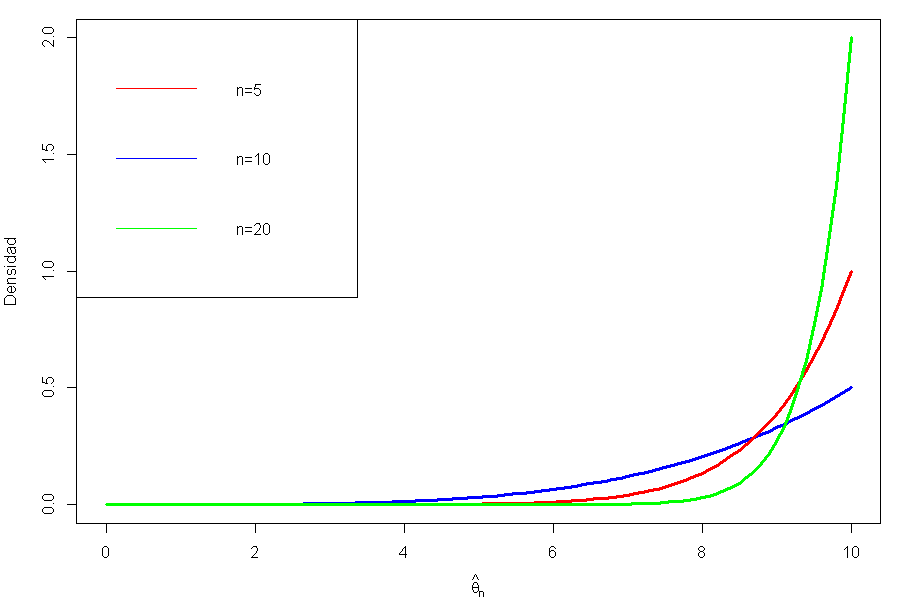
\includegraphics[scale=0.45]{img/consist.png}
    \caption{Distribución de  $\max \{X_1, \cdots, X_n\}$ para distintos valores de $n$ cuando en la población $X\sim U(0,\theta = 10]$.}
\end{figure}

    
\end{frame}

%\begin{frame}{\color{rosee}Convergencia en distribuci\'on}\small
%  \begin{theorem}[TCL]
 %   Sea $X_{1},\dots,X_n$ una muestra aleatoria tal que $E(X)=\mu$ y
  %  $Var(X)=\sigma^{2}$, entonces, para todo $z\in\mathbb{R}$
   % \[P\left(\frac{\sqrt{n}\,(\overline{X}_n-\mu)}{\sigma} \leq z \right)
    %\ton \Phi(z),\]
    %donde $\Phi(z)=P(Z\leq z)$ para $Z \sim N(0,1)$.
  %\end{theorem}
%\end{frame}

% \begin{frame}{\color{rosee}Teorema Central del L\'imite}
%   \small
%   \begin{alertblock}{Idea}
%     Para tama\~nos de muestra grande, la distribuci\'on de
%     $\overline{X}_n$ es aproximadamente normal.
%     $$
%     \frac{\sqrt{n}\,(\overline{X}_n-\mu)}{\sigma} \approx N(0,1)
%     $$
%     y
%     $$
%     \overline{X}_n \approx N\left( \mu, \frac{\sigma^{2}}n
%     \right).
%     $$
%     \medskip
%     
%     El TCL nos dice que, una versi\'on debidamente re-escalada de
%     $\overline{X}_n$ converge en cierto sentido a una normal
%     $N(0,1)$.
%   \end{alertblock}
% \end{frame}

%\begin{frame}{\color{rosee}Convergencia en distribuci\'on}\small
 % \begin{alertblock}{Idea}
  %  Para tama\~nos de muestra grande, la distribuci\'on de
   % $\overline{X}_n$ es aproximadamente normal:
    %\[\frac{\sqrt{n}\,(\overline{X}_n-\mu)}{\sigma} \approx N(0,1)\]
    %y
    %\[\overline{X}_n \approx N\left( \mu, \frac{\sigma^{2}}{n} \right)\,.\]
    %El TCL nos dice que la distribuci\'on de una versi\'on debidamente
    %re-escalada de $\overline{X}_n$ converge en cierto sentido a una
    %normal $N(0,1)$.
  %\end{alertblock}
%\end{frame}

\begin{frame}{\color{rosee}Convergencia en distribuci\'on}\small
  
    Sea \small{$V_{1},\dots,V_n,\dots$} una sucesi\'on de variables aleatorias
    y  $V$ una variable aleatoria. Decimos que la sucesión $(V_n)_{n\in\NN}$ \textbf{converge en
    distribuci\'on a} $V$ si vale
    que\footnote{Para todo $v$ de manera que $F_{V}(v)$ es continua en el punto $v$.}
    \[F_{V_n}(v)=P(V_n\leq v) \ton F_V (v)=P(V \leq v)\,.\]
    
    Para denotar esta convergencia usaremos la notación: $V_n \stackrel{d}{\to} V$.
  
    \begin{alertblock}{\color{rosee}Observaci\'on}
    El TCL  para $X_i\stackrel{iid}{\sim}$ es una herramienta que permite mostrar que $\sqrt{n}(\overline{X}_n-E(X))\cw N(0,Var(X))$ para el caso particular donde la sucesión $V_n=\sqrt{n}(\overline{X}_n-E(X))$ y $V$ tiene distribución $N(0,Var(X))$. 
  \end{alertblock}
  
%  \begin{block}{Notaci\'on}
%    Usaremos la notaci\'on $V_n \cw V$. Tambi\'en haremos el siguiente
%    abuso de notaci\'on. Por ejemplo, si $V\sim N(0,1)$,
%    escribiremos
%    \[V_n \cw N(0,1),\]
%    o, si $V\sim Pois(\lambda)$, escribiremos
%    \[ V_n \cw Pois(\lambda), etc\,.\]
%  \end{block}
\end{frame}

\begin{frame}{\color{rosee} Propiedades de la convergencia en distribución}
\small
\begin{itemize}

\item \textbf{Lema de Slutsky}
  
    Sea $c\in\mathbb{R}$ una constante. Si $W_n \cp c$ y $V_n\cw V$
    entonces
    \[W_n V_n \cw c V \quad \text{ y } \quad V_n+ W_n \cw V +c\]
  
    \item \textbf{Teorema de la función continua}

 Las funciones continuas conservan los límites aún cuando sus argumentos son (sucesiones de) variables aleatorias. En otras palabras, si $g:\mathbb{R}\to\mathbb{R}$ es una función continua y:\medskip

\begin{itemize}
\item $V_{n} \cp c$ entonces $g(V_{n})\cp g(c)$.\medskip

\item $V_{n} \cw V$ entonces $g(V_{n})\cw g(V)$.\medskip
\end{itemize}
\item \color{rosee}\textbf{Ojo!} \color{black} No es cierto que si $V_n\cw V$ y $W_n\cw W$ entonces
    $V_n\cdot W_n\cw V\cdot W$ o $V_n+W_n \cw V+W$. Por ejemplo si $V_n=W_n=V\sim N(0,1)$ y $W=-V\sim N(0,1)$ se tiene que $V_n\cw V$, $W_n\cw W$, pero $V_n+W_n\sim N(0,4)$ mientras que $V+W=0$.
    \end{itemize}
\end{frame}


\begin{frame}{\color{rosee}Ejercicios de convergencia en distribución}
  \begin{exampleblock}{Ejercicio I}
    Sea $X_{1},\dots,X_n\stackrel{iid}{\sim}$ una muestra aleatoria tal que $E(X_1)=0$ y
    $E(X_1^2)=2$. Calcule los l\'imites en distribuci\'on de
    \[Y_n=\frac{\sqrt{n}\, \displaystyle\sum_{i=1}^nX_{i}
    }{\sum\limits_{i=1}^nX_{i}^{2}}\,.\]
    y de
    $$
    W_{n}=e^{Y_{n}}.
    $$
  \end{exampleblock}
  
  \begin{exampleblock}{Ejercicio II}
Resuelva el inciso 5 del ejercicio 5 del TP2.
  \end{exampleblock}
\end{frame}

\begin{frame}{\color{rosee} Estimadores asintóticamente normales}\small
\begin{itemize}
    \item Decimos que $\widehat{\theta}$ es un \textbf{estimador asintóticamente} normal de $\theta$ si existe una expresión que depende de $\theta$, $V(\theta)$\footnote{$V(\theta)$ \textbf{no es} 1) la varianza de $\theta$ (que es cero) \textbf{ni} 2) la varianza de $\widehat{\theta}$.}, que cumple que:
    \[\dfrac{\sqrt{n}(\widehat{\theta}-\theta)}{\sqrt{V(\theta)}}\cw N(0,1)\]
   \item Notemos que la normalidad asintótica es una \textbf{propiedad asintótica} del estimador porque se define para $n\to+\infty$. 
    \item Notar que el TCL para $X_i\stackrel{iid}{\sim}$ vale que \[\dfrac{\sqrt{n}(\overline{X}_n-E(X))}{\sqrt{Var(X)}}\cw N(0,1)\]
    Es decir que $\dfrac{\sqrt{n}(\overline{X}_n-E(X))}{\sqrt{Var(X)}}$ (o $\overline{X}_n$, se puede decir de ambas maneras) es un \textbf{estimador asintóticamente normal} de $E(X)$.
    \end{itemize}
\end{frame}


%\begin{frame}{\color{rosee}Convergencia en dist. vs. convergencia en prob.}
%\small
%\begin{center}
%    Si $V_n \cp V$, entonces $V_n \cw V$.
%\end{center}
%
%    En general no es necesariamente cierto que si $V_n \cw V$ entonces $V_n \cp V$. 
    
 %   \bigskip En otras palabras, la convergencia en distribuci\'on es m\'as \textbf{d\'ebil}
 %   que la convergencia en probabilidad.
  
%  \vspace{6pt}
  
%  Consideremos una v.a. continua $X$ con una funci\'on de probabilidad puntual $f_{X}(x)$ que cumpla ser una funci\'on par, es decir, $f_{X}(x)=f_{X}(-x)$. Se sigue que $-X$ tiene la misma PDF. Definimos la sucesi\'on $V_{n}=X$ si $n$ es impar y $V_{n}=-X$ si $n$ es par, y sea $V=X$, entonces $F_{V_{n}}(z)=F_{V}(z)$ para todo $z$ porque la PDF dw $X$ y $-X$ son iguales. Entonces, $V_{n} \stackrel{d}{\rightarrow} V$. Sin embargo, $V_{n} \stackrel{p}{\rightarrow} V$ porque $Z_{N}$ oscila entre $X$ y $-X$. Son v.a. diferentes, aunque tengan la misma CDF, porque 
%  \[P(X=-X)=P(\{\omega: X(\omega)=-X(\omega)\})=P(\{\omega: X(\omega)=0\})=0\]
%\end{frame}

\begin{frame}{\color{rosee}Normalidad asintótica de $\overline{X}_n$}\small

Si queremos estimar $E(X)$ usando $\overline{X}_n$, sabemos por el TCL para $X_i\stackrel{iid}{\sim}$ que \[\dfrac{\sqrt{n}(\overline{X}_n-E(X))}{\sqrt{Var(X)}}\cw N(0,1)\]

Aquí nos surge una segunda dificultad: podemos estimar puntualmente $E(X)$ usando el estimador $\overline{X}_n$ pero no sabemos cuál es la precisión de dicha estimación porque $\sqrt{Var(\overline{X}_n)}=\sqrt{\dfrac{Var(X)}{n}}$ y no conocemos $Var(X)$.

Vimos en la slide \S6 que $\widehat{\sigma}^{2}$ es un estimador consistente de $Var(X)$, o sea,
  \[\widehat{\sigma}^{2}= \frac{1}{n}\sum\limits_{i=1}^nX_{i}^{2} - 
  \overline{X}_n^{2} \cp Var(X)\]
  
  Por lo tanto, 
  
  \[\widehat{\sigma} =\sqrt{\frac{1}{n}\sum\limits_{i=1}^nX_{i}^{2} - 
  \overline{X}_n^{2}}\cp \sqrt{Var(X)}.\]
  
 
\end{frame}



\begin{frame}{\color{rosee}Normalidad asintótica de $\overline{X}_n$}
 
  Como $\widehat{\sigma} \cp \sqrt{Var(X)}$ eso implica, por las propiedades de convergencia en probabilidad que
  \[\frac{\sqrt{Var(X)}}{\widehat{\sigma}} \cp 1.\] 
  
  Escribiendo
  \[\frac{\sqrt{n}\,(\overline{X}_n-E(X))}{\widehat{\sigma}} =
  \underbrace{\frac{\sqrt{n}\,(\overline{X}_n-E(X))}{\color{rosee}\sqrt{Var(X)}}}_{\cw
    N(0,1) } \underbrace{\frac{\color{rosee}\sqrt{Var(X)}}{\widehat{\sigma}}
  }_{\cp 1} \cw N(0,1),\] por el lema de Slutsky.
  
  Eso quiere decir que si bien no conocemos la precisión $\sqrt{Var(\overline{X}_n)}$ con la que estimamos a $E(X)$ usando $\overline{X}_n$ podemos aproximarla por $\frac{\widehat{\sigma}}{\sqrt{n}}$.
\end{frame}




%\begin{frame}{\color{rosee}Convergencia en distribuci\'on}
%  \begin{alertblock}{\color{rosee}Ojo!}


 %   \bigskip Por ejemplo, sea $V$ con distribuci\'on
 %   $N(0,1)$. Definamos $V_n=V$ y $W_n=V$ para todo $n$ y
  %  $W=-V$.

  %  \bigskip Notemos que
  %  $W\sim N(0,1)$. Entonces
  %  \[V_n \cw V, \quad W_n \cw W\]
  %  pero
  %  \[V_n+W_n=2V \sim N(0,4)\]
  %  y
  %  \[V+W = 0\,.\]
  %\end{alertblock}
%\end{frame}




\begin{frame}{\color{rosee} Método Delta}
\small
\begin{itemize}
    \item No siempre va a ser posible mostrar que un estimador es asintóticamente normal\footnote{De hecho, no todos los estimadores son asintóticamente normales. Por ejemplo, si $X_i\stackrel{iid}{\sim} U(0,\theta]$ se tiene que $n(\theta -\max\{X_1, \cdots , X_n\}) \cw Exp\left(\frac{1}{\theta}\right)$. No vamos a ver muchos de estos casos en el curso.} usando TCL para una muestra aleatoria.
    
    \item ¿Por qué sucede esto? Porque no todos los estimadores son promedios de variables iid.
\end{itemize}
     
 Proposición (Método Delta): Supongamos que $\widehat{\theta}_{n}$ es un estimador asintóticamente normal de $\theta$, es decir,
    $$
    \sqrt{n} \left( \widehat{\theta}_{n} - \color{rosee}\theta\color{black}) \right) \cw N(0,
    V(\theta)).
    $$
    Supongamos que $g(x)$ es una funci\'on con derivada continua y que
    $g^{\prime}(\color{rosee}\theta\color{black}))\neq 0$. Entonces por el Método Delta vale que
    \[\sqrt{n} \left[ g(\widehat{\theta}_{n}) - g(\color{rosee}\theta\color{black})) \right] \cw N[0,
    V(\theta) (g^{\prime}(\color{rosee}\theta\color{black}))^{2}].\]

\end{frame}

\begin{frame}{\color{rosee} Ejercicio con TCL y método delta}\small
    Considere una muestra $X_i\stackrel{iid}{\sim}$, se tiene que $E(X)=\frac{1}{2}\theta$, $E(X^2)=\frac{3}{2}\theta$, $E(X^4)=\frac{5}{2}\theta$, $E(\ln(X))=\ln\left(\frac{1}{3}\theta\right)$ y $E(\ln(X)^2)=\left[\ln\left(\frac{1}{4}\theta\right)\right]^2$, donde $0<\theta<1$. Diga cuál es el límite en distribución de
    
    \begin{enumerate}[label=(\alph*)]
        \item  $\sqrt{n}\left(\overline{X}_n-E(X) \right)$
        \item  $\sqrt{n}\left(\frac{1}{n}\sum_{i=1}^{n}X_i^2-E(X^2) \right)$
        \item  $\sqrt{n}\left[\frac{1}{n}\sum_{i=1}^{n}\ln(X_i)-E(\ln(X)) \right]$
        \item  $\sqrt{n}\left[(\overline{X}_n)^2-E(X)^2 \right]$
        \item  $\sqrt{n}\left[\ln(\overline{X}_n)-\ln(E(X)) \right]$
        \item  $\sqrt{n}\left(\frac{1}{n}\sum_{i=1}^{n}\frac{X_i}{3}-\frac{E(X)}{3} \right)$
        \item Compare los resultados que utilizó para responder a los incisos (b) y (d).
        \item Compare los resultados que utilizó para responder a los incisos (c) y (e).
        \item ¿De qué maneras puede justificar el resultado en (f)?
    \end{enumerate}
\end{frame}

\begin{frame}{\color{rosee}Ejercicio con TCL y método delta (solución)}\small\color{gray}
    \begin{enumerate}[label=(\alph*),leftmargin=*]
        \item Por TCL para $X_i\stackrel{iid}{\sim}$ $\sqrt{n}\left(\overline{X}_n-\frac{1}{2}\theta \right) \stackrel{D}{\to} N\left(0,\frac{3}{2}\theta-\frac{1}{4}\theta^2\right)$, $Var(X)=\frac{3}{2}\theta-\frac{1}{4}\theta^2$
        \item Por TCL para $X_i^2\stackrel{iid}{\sim}$ $\sqrt{n}\left(\frac{1}{n}\sum_{i=1}^{n}X_i^2-\frac{3}{2}\theta \right) \stackrel{D}{\to} N\left(0,\frac{5}{2}\theta-\frac{9}{4}\theta^2\right)$, $Var(X^2)=\frac{5}{2}\theta-\frac{9}{4}\theta^2$
        \item Por TCL para $\ln(X_i)\stackrel{iid}{\sim}$ $\sqrt{n}\left[\frac{1}{n}\sum_{i=1}^{n}\ln(X_i)-\ln\left(\frac{1}{3}\theta\right) \right]\stackrel{D}{\to} N\left[0,Var(\ln(X))\right]$, $Var(\ln(X))=(\ln(4))^2+(\ln(2))^2-2\ln(2)\cdot \ln(\theta)$
        \item A partir de (a), por método delta para $g(x)=x^2$, $g'(x)=2x$, $g'\left(\frac{1}{2}\theta\right)=\theta$,  vale que $\sqrt{n}\left[(\overline{X}_n)^2-\frac{1}{4}\theta^2 \right]\stackrel{D}{\to}N\left(0,\frac{3}{2}\theta^3-\frac{1}{4}\theta^4\right)$
         \item A partir de (a), por método delta para $g(x)=\ln(x)$, $g'(x)=1/x$, $g'\left(\frac{1}{2}\theta\right)=\frac{2}{\theta}$, vale que $\sqrt{n}\left[\ln(\overline{X}_n)-\ln\left(\frac{1}{2}\theta\right) \right]\stackrel{D}{\to}N\left(0,\frac{6}{\theta}-1\right)$
    \end{enumerate}
\end{frame}

\begin{frame}{\color{rosee}Ejercicio con TCL y método delta (solución)}\small \color{gray}
    \begin{enumerate}[label=(\alph*),leftmargin=*]
    \setcounter{enumi}{5}
    \item A partir de (a), por método delta para $g(x)=1/3x$, $g'(x)=1/3$, $g'(\theta/2)=1/3$ vale que $\sqrt{n}\left(\frac{1}{n}\sum_{i=1}^{n}\frac{X_i}{3}-\frac{1}{6}\theta \right)\stackrel{D}{\to}N\left(0,\frac{1}{6}\theta-\frac{1}{36}\theta^2\right)$.

    \vspace{4pt}

    También se podría justificar que vale el resultado por TCL para $\frac{1}{3}X_i\stackrel{iid}{\sim}$ $\sqrt{n}\left(\frac{1}{n}\sum_{i=1}^{n}\frac{X_i}{3}-\frac{1}{6}\theta \right)\stackrel{D}{\to}N\left(0,\frac{1}{6}\theta-\frac{1}{36}\theta^2\right)$ ya que $Var\left(3X\right)=\frac{1}{6}\theta-\frac{1}{36}\theta^2$
    \item La diferencia más importante en (b) y (d) es que en (b) primero elevamos cada v.a. $X_i$ al cuadrado y después las promediamos; mientras que en (d) primero promediamos las variables $X_i$ y luego al promedio lo elevamos al cuadrado. Por esa razón la justificación difiere radicalmente en cada caso.
    \item En los incisos (c) y (e) es análogo a los casos (b) y (d) respectivamente si consideramos que en vez de elevar al cuadrado, tomamos logaritmo.
    \item En el inciso (f), como la función es lineal $g(x)=\frac{1}{3}x$, en este caso tomar promedio y aplicar la función $g$ a $\overline{X}_n$ o primero aplicar la función $g$ a cada dato $X_i$ y después promediar las v.a. $g(X_i)$ da el mismo resultado. Por lo tanto, se puede justificar usando TCL para $g(X_i)\stackrel{iid}{\sim}$ \'o TCL para $X_i\stackrel{iid}{\sim}$ + método delta para $g(x)$.
    \end{enumerate}
     \end{frame}

\begin{frame}[noframenumbering]{}
    \begin{center}
        \Large Apéndice: las slides a partir de aquí son optativas
    \end{center}
\end{frame}

\begin{frame}[noframenumbering]%{\color{rosee}Propiedades de la convergencia en probabilidad}\small
  \begin{proof}
  \textcolor{gray}{
    Probamos (3) (es un buen ejercicio tratar de demostrar las restantes). Sea $\varepsilon>0$. Tenemos que ver que
    \[P\left(\left\vert V_n+W_n -(c_v+c_w) \right\vert\geq \varepsilon \right) \ton 0\,.\]
    Notemos que 
    \[\left\lbrace\left\vert V_n+W_n -(c_v+c_w) \right\vert\geq \varepsilon
    \right\rbrace \subset \left\lbrace\left\vert V_n-c_v \right\vert\geq
      \varepsilon/2 \right\rbrace \cup \left\lbrace\left\vert W_n-c_w
      \right\vert\geq \varepsilon/2 \right\rbrace\,.\]
    Entonces 
    \begin{align*}
      P\left(\left\vert V_n+W_n -(c_v+c_w) \right\vert\geq \varepsilon \right) 
      \leq P\left(\left\vert V_n-c_v \right\vert\geq \varepsilon/2  \right)  +
      \\  P\left(\left\vert W_n-c_w \right\vert\geq \varepsilon/2  \right).
    \end{align*}
    Como $V_n\cp c_v$ y $W_n\cp c_w$
    \[P\left(\left\vert V_n-c_v \right\vert\geq \varepsilon/2 \right) +
    P\left(\left\vert W_n-c_w \right\vert\geq \varepsilon/2 \right) \ton
    0\,.\]
    }
  \end{proof}
\end{frame}

\begin{frame}[noframenumbering]{\color{rosee}Demostraci\'on de que $\widehat{\theta}_n\cmc \theta$ entonces vale $\widehat{\theta}_n \cp \theta$}
\small
\textbf{Caso 1:} Suponemos que $E(\widehat{\theta}_n)=\theta$ para todo $n$. Sea $\varepsilon>0$. Por Markov
    \[P(\left\vert \widehat{\theta}_n -\theta \right\vert \geq \varepsilon)=P(\left\vert \widehat{\theta}_n -\theta \right\vert^2 \geq \varepsilon^2)\leq \dfrac{E\left((\widehat{\theta}_n-\theta)^2\right)}{\eps^2}=
    \frac{Var(\widehat{\theta}_n)}{\varepsilon^{2}} \ton 0\,.\]
  
\textbf{Caso 2, caso general ($E(\widehat{\theta}_n)\neq\theta$):} Sea $\varepsilon>0$. Por Markov


\begin{align*}
    P(&\left\vert \widehat{\theta}_n -\theta \right\vert \geq \varepsilon)=P(\left\vert \widehat{\theta}_n -\theta \right\vert^2 \geq \varepsilon^2)\leq \dfrac{E\left((\widehat{\theta}_n-\theta)^2\right)}{\eps^2}\\
    \leq& \dfrac{1}{\eps^2}E\left((\widehat{\theta}_n\color{rosee}-E(\widehat{\theta}_n)+E(\widehat{\theta}_n)\color{black}-\theta)^2\right)\\
   =&\dfrac{1}{\eps^2}\left(\color{dodgerblue}E\left[\widehat{\theta}_n-E(\widehat{\theta}_n)^2\right]\color{black}-2\color{gren}E\left[(\widehat{\theta}_n-E(\widehat{\theta}_n))(E(\widehat{\theta}_n)-\theta)\right]\color{black}+\color{rosee}E\left[(E(\widehat{\theta}_n)-\theta)^2\right]\color{black}\right)\\
   =&\dfrac{1}{\eps^2} \left(\color{dodgerblue}Var(\widehat{\theta}_n)\color{black}-2\color{gren}\underbrace{(E(\widehat{\theta}_n)-\theta)}_{\text{constante}}\cdot \underbrace{E\left[\widehat{\theta}_n-E(\widehat{\theta}_n)\right]}_{=0}\color{black}+\color{rosee}(E(\widehat{\theta}_n)-\theta)^2\color{black}\right)\ton 0
\end{align*}
 
 %   Lo hacemos suponiendo que $E(V_n)=c$ para todo $n$. 

  %  \bigskip Fijemos $\varepsilon>0$. Por Markov
   % \[P(\left\vert \widehat{\theta}_n -\theta \right\vert \geq \varepsilon)=P(\left( \widehat{\theta}_n -\theta \right)^2 \geq \varepsilon^2)\leq
   % \frac{E\left(\left(\widehat{\theta}_n-\theta\right)^2\right)}{\varepsilon^{2}} \ton 0\,.\]

\end{frame}


\begin{frame}[noframenumbering]{\color{rosee}Convergencia en distribuci\'on}
%  \begin{alertblock}{Idea}
    Si $V_n\cw V$, la funci\'on de distribuci\'on acumulada de $V_n$
    est\'a ``cerca'' de la distribuci\'on de $V$ para valores de $n$
    grandes.

    \medskip\textbf{Esto no quiere decir que $V_n$ est\'e cerca de $V$!}\small

    \medskip De hecho, $V_{1},\dots, V_n$ y $V$ pueden estar definidas
    todas sobre espacios muestrales distintos!

    \medskip La convergencia en distribuci\'on, m\'as que una
    convergencia de variables aleatorias, \textbf{es una convergencia de
    funciones de distribuci\'on}. De hecho, si llamamos $F_{V_n}$ a la
    funci\'on de distribuci\'on de $V_n$ y $F_{V}$ a la funci\'on de
    distribuci\'on de $V$, $V_n\cw V$ si
    \[F_{V_n}(v) \ton F_{V}(v)\]
    para todo $v$ donde $F_{V}$ es continua.
    
    \textbf{Por ejemplo, }si las variables $X_i\sim_{iid} Be(p)$, $n\overline{X}_n$ tiene distribución $Bin(n,p)$ que toma $n+1$ valores. Por lo tanto, 
    $\sqrt{n}(\overline{X}_n-p)$ también toma $n+1$ valores. Sin embargo, $\sqrt{n}(\overline{X}_n-p)\cw N(0,Var(X))$ donde la distribución normal toma infinitos posibles valores.
%  \end{alertblock}
\end{frame}

\begin{frame}[noframenumbering]{\color{rosee}¿Por qu\'e pedimos convergencia s\'olo donde
      $F_{V}$ es continua?}
      
      Este es un detalle técnico que es importante pero que no nos afecta en los ejemplos que vemos la materia. Por eso no nos detenemos en profundidad. Eso no quiere decir que este detalle no sea importante.
  \begin{alertblock}{}


    Consideremos $V_n$ tal que $P(V_n=1/n)=1$ y sea $V$ tal que
    $P(V=0)=1$. Intuitivamente, esperar\'iamos que $V_n\cw V$.

    \medskip La funci\'on de distribuci\'on acumulada de $V$ tiene una
    discontinuidad en 0. Ahora
    \[P(V_n\leq 0) =0 \quad y \quad P(V\leq 0)=1\]
    en particular
    \[P(V_n\leq 0) \nrightarrow P(V\leq 0)\,.\]
    Sin embargo, es f\'acil mostrar que efectivamente $V_n \cw V$, ya
    que $0$ es el \'unico punto donde la funci\'on de distribuci\'on
    acumulada de $V$ tiene una discontinuidad.
  \end{alertblock}
\end{frame}

\end{document}
